\section{Above and Below}
\label{above-and-below}

We now describe the tooling we have built \emph{above}
the Graffiti API that makes development even easier, and
the implementations we have built \emph{below} the API
that realize different trade-offs between efficiency and
robustness.

While we have made insights on both fronts that at
the least demonstrate \emph{feasibility},
there are, of course,
many unanswered questions and unexplored ideas.
Fortunately, by having a fixed API in the middle, work done above the API
is \emph{decoupled} from work done below.
It is possible to drop in a new, more efficient, or privacy-preserving implementation
without upheaving all the tools and applications that have been built on top.

\subsection{Above}

While the API has hidden significant complexity below,
like the need to write and deploy server code or the need to
consider the server infrastructure at all,
writing front-end code is still inaccessible
to many people.
We have made some initial steps toward reducing the
programming complexity by allowing for the \emph{reactive} and
\emph{declarative} programming of Graffiti applications
and by providing a growing library of reusable design patterns.
We also point to a future where Graffiti applications could be built
without any code at all.

\subsubsection{Vue Plugin}

Vue is a popular front-end framework that enables ``reactive'' programming where
changes to the underlying state are automatically reflected in the UI.
We built a plugin for Vue\footnote{
  \url{https://vue.graffiti.garden/variables/GraffitiPlugin.html}
}
that provides a variant of
\texttt{discover} which returns a reactive array of objects rather than
an asynchronous stream.
Any CRUD operation that the user triggers locally instantly updates
the relevant array, while remote changes can be polled manually
with \texttt{poll()} or automatically
with an \texttt{autopoll} setting.

This reactivity is available in a traditional programming
environment as well as in a declarative HTML-like template.
The plugin maintains complete TypeScript support and
is a relatively light wrapper over a Graffiti-specific reactivity library we have developed\footnote{
   \url{https://sync.graffiti.garden/classes/GraffitiSynchronize.html}
}.
Therefore, support for other front-end frameworks, like React, will be
fairly easy to add in the future.

Below is the complete template for a micro social application,
built with the plugin, that shows a (continuously updating) list of all messages posted to a real-time group chat and enables the user to post their own message:
\begin{minted}{vue}
<form v-if="$graffitiSession.value"
  @submit.prevent="$graffiti.put({
    value: { content },
    channels: [ 'my-group' ]
  }, $graffitiSession.value)"
>
  <input v-model="content" />
  <input type="submit" value="Post" />
</form>
<button v-else @click="$graffiti.login()">
  Log In to Post!
</button>
<GraffitiDiscover autopoll
  v-slot="{ objects: messages }"
  :channels="[ 'my-group' ]"
  :schema="{
    properties: {
      value: {
        required: ['content'],
        properties: {
          content: { type: 'string' },
        }
      }
    }
  }"
>
  <ul>
    <li v-for="message in messages">
      {{ message.value.content }}
    </li>
  </ul>
</GraffitiDiscover>
\end{minted}

\subsubsection{Pattern Library}

We have started compiling a library of common patterns\footnote{
    \url{https://vue.graffiti.garden/examples/}
} that currently includes likes, profiles, following, threaded comments,
and different messaging patterns.
These patterns build on top of the Vue plugin
and are self-contained in \emph{single HTML files}
which can be downloaded, modified, and copied into other
applications.
Perhaps this format can encourage the copy and paste ``pimp my page''
programming that was once possible on MySpace~\cite{copypasteliteracy},
but with the ability to add new \emph{functionality} rather than just styling.

\subsubsection{Future Work}
\label{above-and-below:above:future-work}

There is certainly potential for more low or even no-code tools
to be developed on top of the Graffiti API. It is an open
question as to whether it is possible to build an intuitive and completely
no-code system for Graffiti, like a graphical editor, without limiting
its extensibility.

Additionally, in our own application development,
we found that inline AI tools like GitHub Copilot are already
capable of generating large portions of functional Graffiti code.
This is especially true when writing applications with the
Vue plugin, perhaps because of the reduction in boilerplate
code and the declarative nature of the templates.
It is not hard to imagine a future where a developer asks
a large language model to ``make a messaging app''
or to ``add a bookmark button to posts in this application'' and
it simply works.

Work could also be done to develop ``meta'' applications.
Users of these applications could easily change their functionality
by swapping out different plugins,
which could represent different feed sorting algorithms
(similar to \cite{threeleggedstool, bluesky}),
different moderation policies, different styles,
or different features.

Alternatively, Graffiti could serve as a new basis for
\emph{computational media}~{\cite{computationalmedia}},
where the boundary between developing and using applications is blurred.
This would require representing Graffiti applications with
Graffiti objects, potentially by extending the
collaborative editing capabilities we demonstrate in Section~{\ref{case-studies:wikiffiti}}.
Graffiti's social focus may fill gaps left by existing computational media
systems like WebStrates~{\cite{webstrates}} and its successors, CodeStrates~{\cite{codestrates}}
and Mirrorverse~{\cite{mirrorverse}}, which provide malleable interactive environments
for small, trusted teams, but have limited affordances
for \emph{moderation} or \emph{discovery} of social content.

\subsection{Below}

The Graffiti API is relatively simple
and so its implementation must solve just two main problems:
storing objects and discovering objects by channel.
One solution is to store all objects on a massive database
and then discovery is trivially a query on that database.
Unfortunately, this centralizes all control of the network
on that single server.

Instead, we explore \emph{decentralized} implementations of the API.
In the ``remote'' implementation, objects are served by a ``federation'' of databases,
each of which is a small version of the would-be centralized database.
In the ``commodity storage'' implementation, the problems of storage and discovery are split up,
with existing providers, similar to Dropbox, handling storage,
and a new entity, called a ``tracker,'' handling discovery.

These implementations have trade-offs, with
the former implementation being more efficient,
and the latter more robust.
Fortunately, multiple implementations can be understood within one \emph{meta}-implementation,
per Requirement~\ref{requirements:parallel-implementations},
allowing new implementations,
with better trade-offs, to be organically adopted without
invalidating all the data served by older implementations.

These parallel implementations are possible because, as we have mentioned, an object's URL starts with a scheme that indicates
how the various CRUD methods should resolve and interact with the object.
For example, if an actor tries to \texttt{delete} an object whose URL starts with the scheme
\texttt{graffiti:remote:}, their meta-implementation will employ the remote implementation,
while if the URL starts with the scheme \texttt{graffiti:cs:},
their meta-implementation will employ the commodity storage implementation.
To handle \texttt{discover}, the meta-implementation simply aggregates
the results of each implementation-specific \texttt{discover}
operation into one stream.

There are two additional questions we need to resolve to
make coexisting implementations work.
Which implementation should be used
when an actor \emph{first} \texttt{put}s an object?
And what \emph{identity} system will work across multiple
implementations?

For the question of first \texttt{put}s, we simply give the user the choice.
The first time a user attempts to \texttt{put} an object,
a popup opens,
as shown in Figure~\ref{above-and-below:figure:choose-protocol},
asking them which implementation they would like to use,
as well as implementation-specific information, such as what server
they want to store their data on.
We have tried to make the experience relatively frictionless, with
reasonable defaults for
users who do not know or care about the underlying infrastructure.
Importantly, this interface is built into the \emph{meta-implementation}
of the API and so it is not the concern of developers building
applications on top of the API.

\begin{figure}[h]
    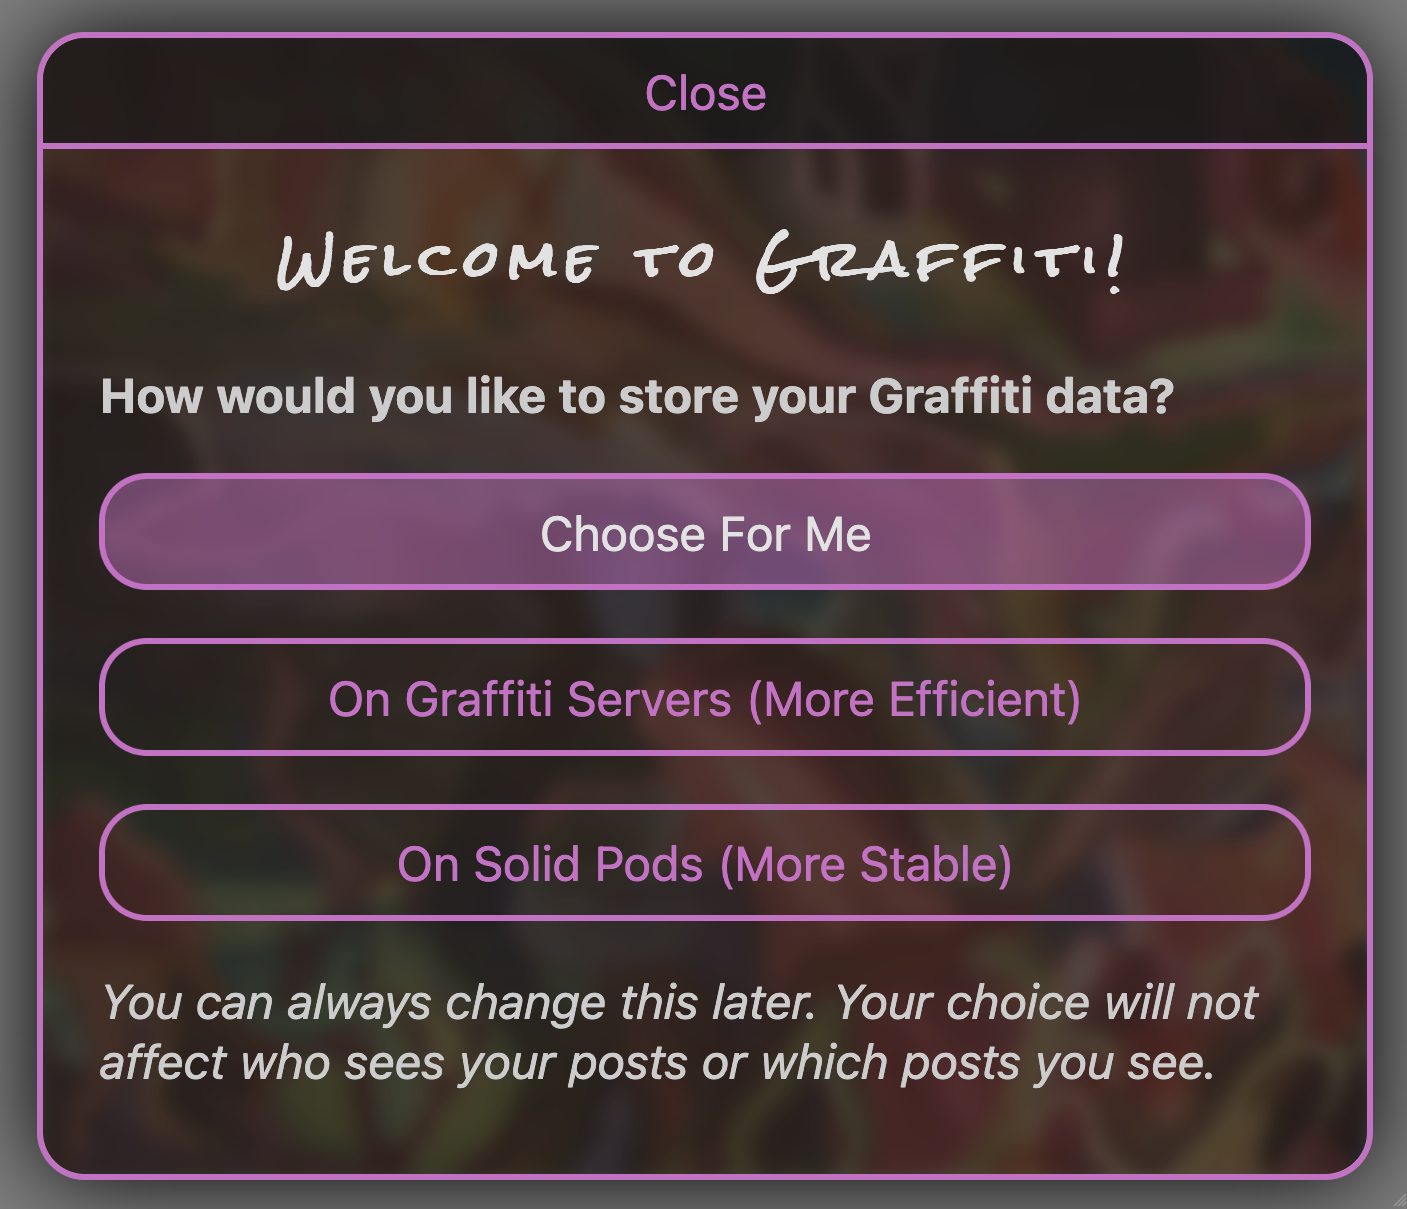
\includegraphics[width=\columnwidth]{figures/choose-protocol.png}
    \caption{The modal that pops up when the user triggers a \texttt{put()} for the first time.}
    \Description{The figure shows a window titled "Welcome to Graffiti!" in a Graffiti-style font. Below a question asks "How would you like to store your Graffiti data?" and three buttons are presented "Choose for Me", "On Graffiti Servers (More Efficient)", and "On Solid Pods (More Stable)". The "Choose for Me" option is emphasized. Below there is a note: "You can always change this later. Your choice will not affect who sees your posts or which posts you see". There is also a close button at the top of the window.}
    \label{above-and-below:figure:choose-protocol}
\end{figure}

As for identity, we currently use a decentralized protocol called Solid OIDC~\cite{solidoidc}.
It has the useful property that a user only needs to log in once
with an ``identity provider'' which then silently authenticates
them with other services.
It is also already used by the Solid protocol~\cite{solid},
which we use in our commodity storage implementation as a ``decentralized Dropbox.''

Unfortunately, Solid OIDC is not a widely deployed and familiar identity solution,
like ``Log in with Google.''
We are keeping an eye on the Decentralized Identifier (DID) specification, which attempts to unify
various identity methods, but, currently, DIDs
do not capture Solid OIDC's property of silent authentication~\cite{dids}.
This would produce a tedious and confusing experience analogous to having to log in every time you receive email from a new server.
We hope that DIDs or new specifications evolve past this restriction.

After discussing our two main implementations, we discuss
a bonus ``utility'' implementation that demonstrates
the additional power of an abstract API.

\subsubsection{Remote Implementation}
\label{above-and-below:remote-protocol}

The remote implementation involves a federation of database servers,
each of which exposes the Graffiti API through an HTTP API.
Like email, users can choose which server they would
like to use or run their own.
Unlike email, the servers do not send objects to each other.
Instead, the client fetches objects directly from servers,
selecting which server to fetch from based on a \emph{domain}
in the object's URL, just as different implementations are selected by \emph{scheme}.

For discovery, we currently provide a registry of servers
and clients call \texttt{discover} on all servers in the registry.
If many servers are deployed, discovering from every one
will be infeasible, and so instead we can use an ``announce''
protocol, detailed in Appendix~\ref{appendix:announce}. The protocol builds on top of the remote implementation,
but only requires the client to
call discover on the servers containing relevant data,
plus a small constant number of well-known
``\emph{rendez-vous}'' servers.

Our server-side software for the remote implementation
consists of a NestJS server with a CouchDB database,
bundled as a Docker image for easy cross-platform
deployment\footnote{
\url{https://github.com/graffiti-garden/implementation-remote}
}.

\subsubsection{Commodity Storage Implementation}
\label{above-and-below:commodity-storage-protocol}

An alternative Graffiti implementation builds on top of existing
\emph{commodity storage} providers,
similar to Dropbox.
Like the remote implementation, users get to choose which storage
service they would like to store their objects in, including
from one they host themselves.
The client software
manages channel-specific files on the storage provider,
each containing all the objects the actor has published to that channel.
The client software shares links to those channel files with a \emph{tracker}.
The tracker is similar to a BitTorrent tracker~\cite{bittorrent} but
rather than mapping torrent IDs to IP addresses
it maps channel strings to channel file URLs.
To run \texttt{discover}, the client software queries the tracker
about each channel of interest and then fetches each of the resulting URLs for objects.

The commodity storage implementation is less efficient than the remote implementation because each
\texttt{discover} call requires a network request per-channel-per-actor,
where as the remote implementation requires only one request per remote server.
If, like email or Mastodon, many actors, especially those in regular contact,
use the same server~\cite{mastodonchallenges},
then \texttt{discover} on the remote implementation can take as
few as \emph{one} request, while requests made by
the commodity storage implementation scale with the number of actors.
Additionally, the schema provided to \texttt{discover} cannot be used for any
server-side filtering---a client must download \emph{all} objects in a channel
and discard ones that do not match the schema.

Still, for users who tend to participate in small networks, these issues
of scale are not a concern and the use of ``simple'' storage servers can be appealing.
The user does not need to worry that an experimental new service
will go offline or lose their data, and we, as implementers do not need to
worry about developing the infrastructure.

At the time of writing, we have built the tracker server and client\footnote{
  \url{https://github.com/graffiti-garden/link-service}\\
  \url{https://github.com/graffiti-garden/link-service-client}\\
  WebTorrent was considered instead of a custom tracker,
  but unfortunately it does not persist announcements more than a few hours.
}, and the complete implementation software,
using Solid ``pods'' as storage providers,
will soon be complete.

\subsubsection{Local Implementation}

This implementation runs entirely client-side
and handles objects with the URL scheme \texttt{graffiti:local:}.
Any data created using the local implementation is only visible on the device on which
it was created.
While such a restriction may seem like a non-starter for an implementation
of our \emph{social} API, it is invaluable for development.
It provides a similar functionality to running a \texttt{localhost} development server,
but
does not require the complexity of standing up a local server.
Developers can easily create test actors and test objects on the local implementation
without polluting their own online presence or existing Graffiti applications.
Finally, the implementation is accessible in deployed applications
and lets users try a Graffiti application out without
having to create or log in to an account, as shown in
Figure~\ref{above-and-below:figure:login}.

\begin{figure*}[t]
    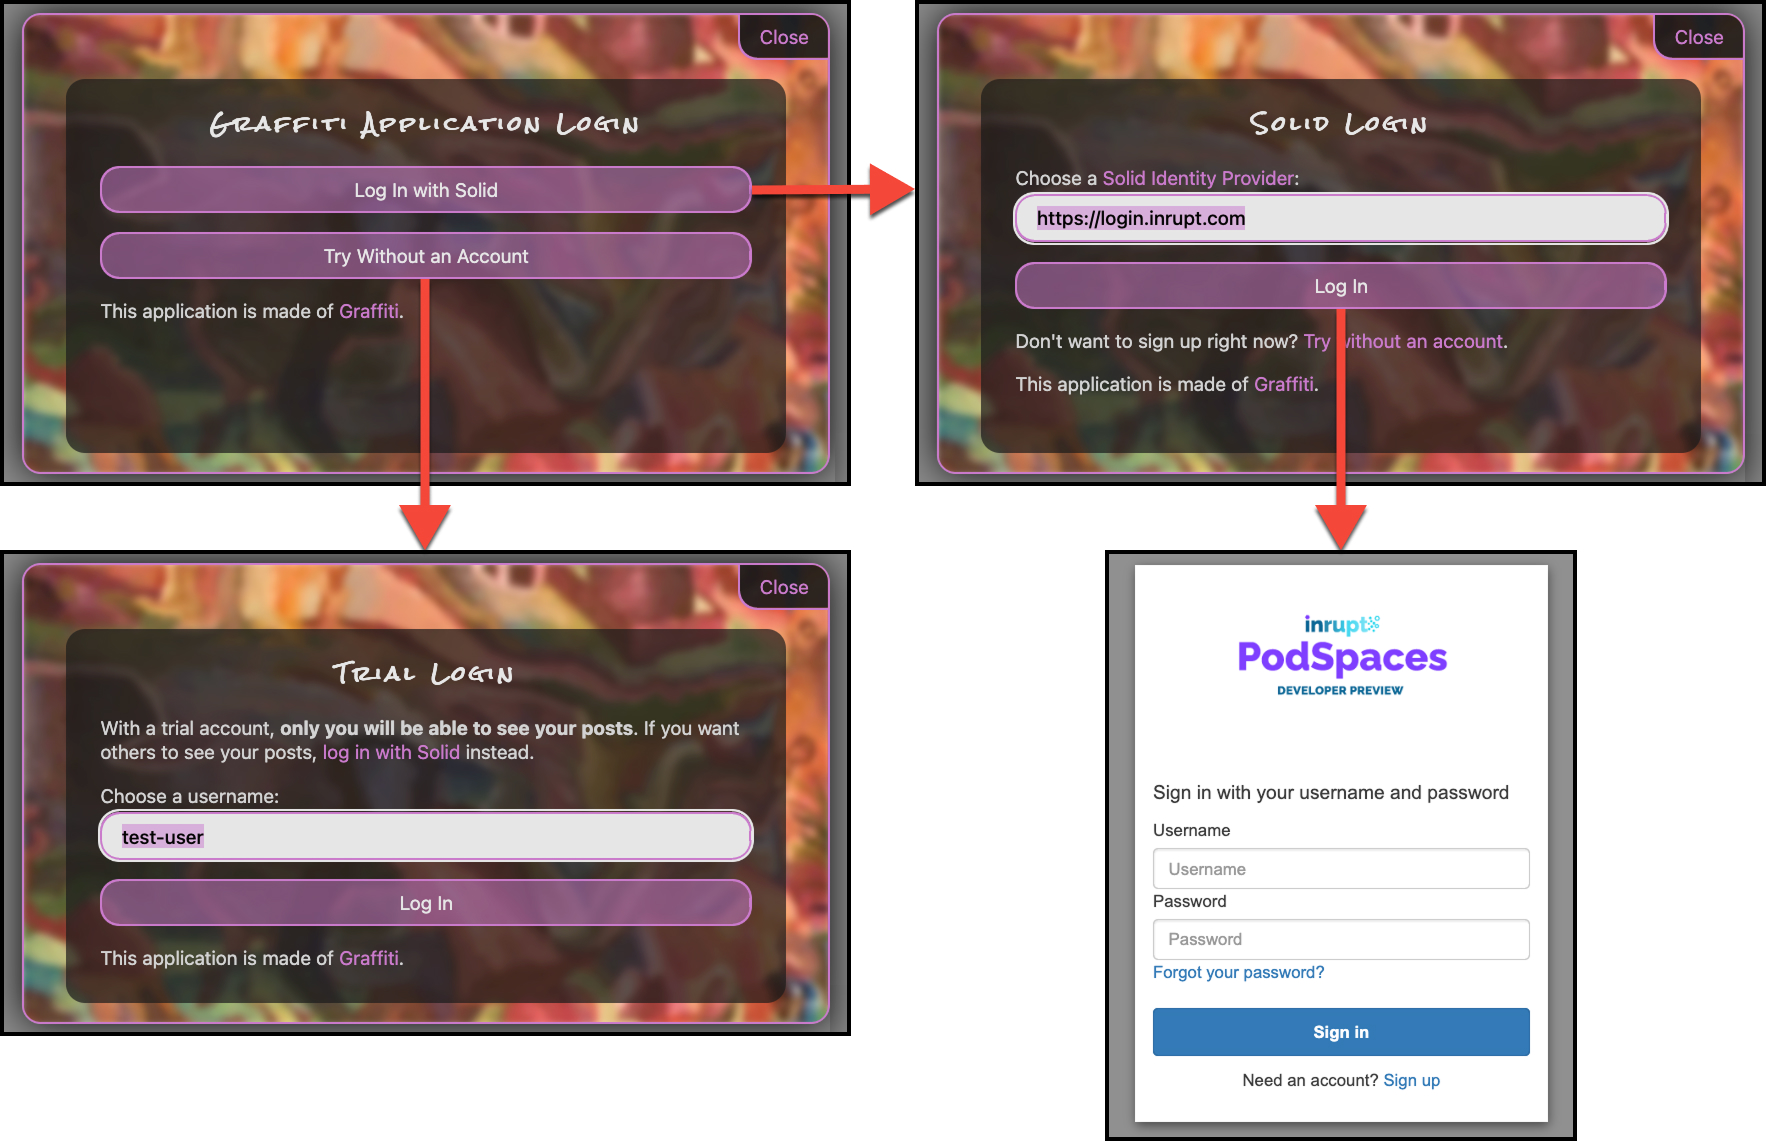
\includegraphics[width=\textwidth]{figures/login.jpg}
    \caption{The flow that pops up when the user triggers a \texttt{login()}.}
    \Description{The figure shows a series of pop-up windows with arrows between them. The first window says "Graffiti Application Login" and below there are buttons to "Log In with Solid" and "Try Without an Account". An arrow pointing from the "Try Without and Account" option points to another window titled "Trial Login" which contains the paragraph "With a trial account, *only you will be able to see your posts*. If you want others to see your posts, log in with Solid instead" and below that a form saying "Choose a username" with "test-user" entered in the input and finally a button to "Log In". From the "Log In with Solid" button in the original panel there is an arrow pointing to a window titled "Solid Login" which says "Choose a Solid Identity Provider" and below an input containing "htttps://login.inrupt.com" and "Log In" and finally "Don't want to sign up right now? Try without an account." An arrow points from the "Log In button of the "Solid Login" window to a new window that looks minimal rather than the more maximalist graffiti designs of the previous windows. This minimal window is titled "inrupt PodSpaces Developer Preview" with the paragraph "Sign in with your username and password" and below a username and password form, text that says "Forgot your password", a "Sign in" button, and finally "Need an account? Sign up".}
    \label{above-and-below:figure:login}
\end{figure*}

Because of its relative simplicity, the local implementation\footnote{
    \url{https://github.com/graffiti-garden/implementation-local}
} serves as the reference implementation of the Graffiti API.


\subsubsection{Future Work}
\label{above-and-below:below:future-work}

The remote implementation offloads object filtering work to complex storage servers,
while the commodity storage implementation shifts that work to clients, keeping the servers simple.
A middle ground is possible by adding more structure to the organization of objects on
the storage servers, and by adding complexity to the tracker to index that structure.
For example, rather than putting all objects in a channel into one file,
those files could be subdivided according to common object schemas.
This would maintain the use of simple servers, but make \texttt{discover} calls more efficient.

In the commodity storage implementation, the tracker also serves as a central point of control and so, like in BitTorrent,
it could be replaced with a distributed hash table~\cite{bittorrentdht}. In small networks,
a tracker may not be necessary at all and can be replaced with a gossip protocol.

Currently each server owner can see all the objects and channels
that pass through it. While federation allows users to switch
to servers they trust, those servers are still vulnerable to
subpoenas, putting groups, like activists, at risk.
It would be valuable to build end-to-end encrypted versions of the remote servers,
tracker, and commodity storage servers, perhaps building on
searchable encryption~\cite{searchableencryption}.

One vulnerability of any system with portable login,
including systems like Solid and the AT Protocol~{\cite{bluesky}},
is the potential of logging into
a malicious application that could steal your data or
post on your behalf without consent.
This risk may make users hesitant to try new applications,
restricting the ecosystem.
Future work should introduce login scopes, such as
the ability to grant an application the permission only to read objects
that match a particular schema and reside in a particular set of channels.
Since the commodity storage implementation bootstraps off of
existing storage services that lack such scoping,
it may be necessary to implement scoping client-side
via an iframe to a trusted intermediary domain.
